\section{Backend}\label{sec:impl_backend}
	V~rámci backendové nebo-li serverové části projektu je prvně nutné zmínit, že funguje na principu API - tzn. že na ní přicházejí požadavky od klienta, na které náležitě odpovídá. Nevrací ani nijak nespravuje vizualizaci dat - jen předává data na frontendovou část, o~které je psáno v~sekci \ref{sec:impl_frontend}.
	
	Zde jsou zobecněné základní úkony, které v~této implementaci právě backend vykonává:
	
	\begin{itemize}
		\item Zpracování a vyřizování požadavků z~webové frontendové části
		\item Administraci databáze - tzn. vytváření, úpravu, mazání a čtení jednotlivých objektů a migrace databáze (tj. automatizovaná deklarace struktury databázových objektu)
		\item Rozesílání emailů (např. pozvánky na neveřejný formulář)
		\item Exportování dat do Excel tabulek
		\item Autentifikaci uživatele
	\end{itemize}
	 
	V~následující části jsou popsány jednotlivé backendové komponenty a principy, díky kterým je celý projekt implementován.
	
	\subsection{Obecná struktura Laravel projektu}\label{sec:strukura_laravel}
	Prvně je nutné rozebrat obecnou strukturu Laravel projektu. 
		\begin{figure}[H]
			\centering %% příkaz, který ti obrázek zarovná na střed
			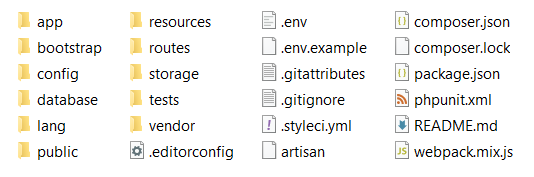
\includegraphics[width=0.9\textwidth]{img/laravel_struktura.png} %% vložení samotného obrátku
			\caption{Obecná struktura nově vygenerovaného Laravel projektu} %% popisek obrázku, nezapomeň na citace!
			\label{fig:laravel_str} %% označení až budeš chtít na obrázek odkazovat
		\end{figure}
	%% obrázek struktury složky
	Jak můžeme na obrázku \ref{fig:laravel_str} vidět, celý projekt je složen z~mnoha složek a souborů. Jelikož podrobný rozbor jednotlivých částí není předmětem této práce, tak jsou nejdůležitější části pro implementaci projektu popsány níže jen obecně.
	\begin{itemize}
		\item Složka \textit{app} obsahuje většinu souborů jádra aplikace (obsahuje např. modely či kontrolery). \cite{LaravelDir}
		\item Složka \textit{bootstrap} obsahuje soubory pro zavedení a spuštění aplikace. \cite{LaravelDir}
		\item Složka \textit{config} obsahuje konfigurace jednotlivých částí aplikace. \cite{LaravelDir}
		\item Složka \textit{database} obsahuje soubory spojené s~prací s~databází. \cite{LaravelDir}
		\item Složka \textit{lang} obsahuje soubory jazyků a překladů (zde nevyužita). \cite{LaravelDir}
		\item Složka \textit{public} obsahuje soubory, které jsou veřejně dostupné při uživatelské interakci s~aplikací (např. při načtení webu v~prohlížeči). \cite{LaravelDir}
		\item Složka \textit{resources} obsahuje pohledy a nezkompilované soubory pro celý frontend. \cite{LaravelDir}
		\item Složka \textit{routes} obsahuje všechny definice cest aplikace (např. cestu \textit{/api/forms/create} pro vyřízení požadavku na vytvoření nového formuláře). \cite{LaravelDir}
		\item Složka \textit{storage} obsahuje primárně záznamy o~chodu aplikace a jiné aplikací vygenerované soubory. \cite{LaravelDir}
		\item Složka \textit{tests} obsahuje automatizované testy aplikace (zde nevyužita). \cite{LaravelDir}
		\item Složka \textit{vendor} obsahuje závislosti a soubory přídavných balíčků spravované Composerem (viz sekce \ref{sec:composer}), které aplikace používá. \cite{LaravelDir}
		\item Soubor .env drží veškeré důležité administrativní hodnoty jako např. přihlašovací údaje k~databázi.
		\item Soubor artisan obsahuje důležité příkazy pro sestavení a spuštění aplikace. \cite{LaravelArtisan}
		\item Soubor composer.json drží informace o~přídavných balíčcích Composeru (viz sekce \ref{sec:composer}) pro Laravel projekt. \cite{ComposerpJSON}
		\item Soubor package.json drží informace o~přídavných balíčcích spravovaných pomocí NPM (viz sekce \ref{sec:npm}) pro frontendovou část projektu. \cite{NPMpJSON}
		\item Soubor webpack.mix.js obsahuje informace pro kompilaci souborů pro frontend. \cite{LaravelJSCSS}
	\end{itemize}

	\subsection{Cesty}\label{sec:routes} %%Routes
	Cesty (volně přeložen původní název Routes) jsou abstraktně využívány k~rozdělení aplikace - to je myšleno tak, že na každé cestě lze provádět jen úkon, který jí je přiřazen. Tyto cesty mají tvar URL adresy - skládají se z~názvu výchozí domény, který je rozšířen o~příslušnou cestu (ve formě textového řetězce děleného lomítky), a jsou využívány např. v~prohlížeči pro přístup na specifickou stránku. Příkladem může být cesta vytvoření formuláře s~příkladovou výchozí doménou \textit{localhost} s~portem 8000 \textit{\uv{localhost:8000/forms/create}}. Po zadání této cesty do webového prohlížeče se za splnění podmínek jako spuštění lokálního serveru s~aplikací a přihlášení do uživatelského účtu zobrazí požadovaná stránka.
	
	Běžně se v~Laravelu tyto cesty definují v~souboru \textit{web.php} - v~tomto projektu tomu tak ale úplně není, jelikož cesty, kam se uživatel může v~aplikaci dostat, jsou definovány ve frontendové části (viz sekce \ref{sec:fe_router}) - to také vyplývá z~předem dané koncepce aplikace - Laravel má sloužit jen jako API, proto neřeší, jaká data budou v~prohlížeči vykreslena - k~tomu slouží frontendová část ve VueJS. K~těmto účelům je ve zmíněném souboru deklarováno, že na jakékoli cestě se má vrátit prázdný pohled \textit{app} (popsán v~části \ref{sec:be_pohledy}), který je pak doplněn o~příslušný obsah, který zajišťuje oddělený frontend (viz obrázek \ref{fig:routes_web}). Jedinou výjimkou jsou zde předdefinované cesty pro resetování hesla pro samotný~Laravel.
	
	\begin{figure}[H]
		\centering %% příkaz, který ti obrázek zarovná na střed
		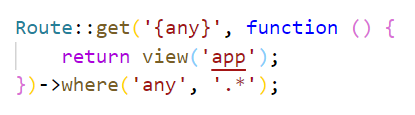
\includegraphics[width=0.6\textwidth]{img/routes/web_routes.png} %% vložení samotného obrátku
		\caption{Část kódu \textit{web.php} vracející pohled \textit{app} na všech cestách} %% popisek obrázku, nezapomeň na citace!
		\label{fig:routes_web} %% označení až budeš chtít na obrázek odkazovat
	\end{figure}
	
	Cesty, které Laravel specificky obsluhuje, jsou v~souboru \textit{api.php} (viz. obrázek \ref{fig:routes_api}). Na tyto cesty uživatel v~adresním řádku webového prohlížeče vůbec nepřistupuje - jsou využívány ve frontendové části na pozadí (viz sekce \ref{sec:komunikace_s_api}). Až zde je vlastně definováno abstraktní rozdělení aplikace - dle cesty se vykonává určitý úkon. 
	
	Tyto API cesty jsou oproti běžným cestám aplikace rozlišeny tak, že mezi výchozí doménu a cestu k~dané službě je vložen řetězec \textit{\uv{/api/}} - to je výchozí chování cest v~souboru \textit{api.php}. K~tomu, aby tyto cesty fungovaly s~dalšími službami, bylo nutné je specifikovat v~konfiguračních souborech \textit{sanctum.php} a \textit{cors.php}.
	
	\begin{figure}[H]
		\centering %% příkaz, který ti obrázek zarovná na střed
		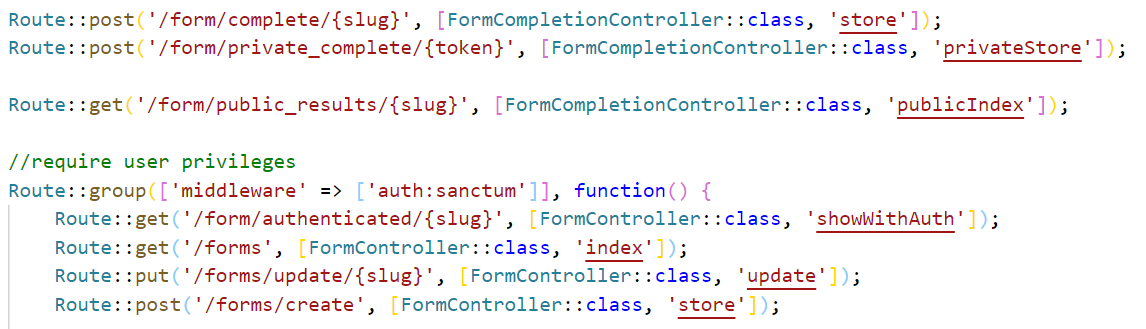
\includegraphics[width=0.9\textwidth]{img/routes/api_routes.png} %% vložení samotného obrátku
		\caption{Část kódu \textit{api.php}} %% popisek obrázku, nezapomeň na citace!
		\label{fig:routes_api} %% označení až budeš chtít na obrázek odkazovat
	\end{figure}
	
	Zmíněné cesty jsou rozděleny do dvou skupin - s~veřejným přístupem (bez přihlášení) nebo s~privátním přístupem (s~přihlášením). Veřejné cesty jsou obslouženy vždy, privátní cesty jsou obslouženy jen pokud jsou společně s~příslušnými daty odeslány údaje o~přihlášení (tj. autorizační tokeny) - ty si autonomně spravuje balíček \uv{Laravel Sanctum} pro zabezpečení single-page aplikací. Ke každé cestě je přidělen úkon (tj. funkce obsahující, co se má s požadavkem provést), který je deklarován v~příslušném kontroléru. 
	
	Zmíněné cesty mají také deklarováno, jakou metodu komunikace používají. V~této implementaci byly využity zejména tyto metody: standardní GET a POST, ale také PUT pro aktualizaci dat nebo DELETE pro mazání dat.
	
	V~rámci popisu aplikace jsou zde tabulky s~jednotlivými cestami a jejich úkony - tabulka \ref{tab:verejne_cesty} obsahuje veřejné cesty a tabulka \ref{tab:cesty_s_prihlasenim} obsahuje cesty s~přihlášením. Hodnoty u~cest ve složených závorkách značí určitou proměnnou přenášenou přes URL adresu (např. \textit{slug} jako identifikátor formuláře).
	
	\newpage
	\begin{table}[H]
		\centering
		\begin{tabular}{ | p{0.4\linewidth} | p{0.1\linewidth} | p{0.4\linewidth} | } 
			\hline
			\textbf{Cesta (\texttt{/api/} + řetězec níže)} & \textbf{Metoda} & \textbf{Funkce} \\ 
			\hline
			\texttt{/login} & POST & Přihlášení uživatele \\ 
			\hline
			\texttt{/register} & POST & Registrace uživatele \\ 
			\hline
			\texttt{/logged\_user} & GET & Vrácení přihlášeného uživatele \\ 
			\hline
			\texttt{/forgot\_password} & POST & Zaslání emailu pro resetování hesla \\
			\hline
			\texttt{/reset\_password} & POST & Resetování hesla \\
			\hline
			\texttt{/form/\{slug\}} & GET & Vrácení veřejného formuláře \\
			\hline
			\texttt{/private\_form/\{token\}} & GET & Vrácení privátního formuláře \\
			\hline
			\texttt{/form/complete/\{slug\}} & POST & Odeslání odpovědi na veřejný formulář \\
			\hline
			\texttt{/form/private\_complete/\{token\}} & POST & Odeslání odpovědi na privátní formulář \\
			\hline
			\texttt{/form/public\_results/\{slug\}} & GET & Vrácení veřejných výsledků formuláře \\
			\hline
		\end{tabular}
		\caption{Veřejné cesty}
		\label{tab:verejne_cesty}
	\end{table}

	\begin{table}[H]
		\centering
		\begin{tabular}{ | p{0.4\linewidth} | p{0.1\linewidth} | p{0.4\linewidth} | } 
			\hline
			\textbf{Cesta (\texttt{/api/} + řetězec níže)} & \textbf{Metoda} & \textbf{Funkce} \\ 
			\hline
			\texttt{/form/authenticated/\{slug\}} & GET & Vrácení formuláře pro administrátorský přístup \\
			\hline
			\texttt{/forms} & GET & Vrácení formulářů, které patří uživateli \\
			\hline
			\texttt{/forms/update/\{slug\}} & PUT & Aktualizace formuláře \\
			\hline
			\texttt{/forms/create} & POST & Vytvoření formuláře \\
			\hline
			\texttt{/forms/\{slug\}} & DELETE & Odstranění formuláře \\
			\hline
			\texttt{/form/duplicate} & POST & Duplikování formuláře \\
			\hline
			\texttt{/form/results/\{slug\}} & GET & Vrácení výsledků formuláře \\
			\hline
			\texttt{/form/results/\{slug\}/download} & GET & Export výsledků formuláře ke stažení \\
			\hline
			\texttt{/form/results/\{slug\}/\newline publish\_results} & POST & Nastavení veřejných výsledků \\
			\hline
			\texttt{/forms/update\_access/\{slug\}} & PUT & Úprava přístupu k~formuláři \\
			\hline
			\texttt{/logout} & POST & Odhlášení uživatele \\
			\hline
			\texttt{/change\_password} & PUT & Změna hesla \\
			\hline
			\texttt{/delete\_account} & POST & Smazání účtu uživatele \\
			\hline
		\end{tabular}
		\caption{Cesty s~přihlášením}
		\label{tab:cesty_s_prihlasenim}
	\end{table}
	\newpage
	
	\subsection{Modely}
	Modely slouží k~mapování jednotlivých dat z~databáze a jsou zprostředkovány pomocí objektově-relačního mapovacího balíčku Eloquent. Pro správnou funkčnost musí být zajištěno, že má každá tabulka v~databázi vlastní model. Díky tomuto přístupu lze s~daty manipulovat tak, že vytvoříme instanci příslušné třídy a na ní voláme příslušné metody (např. \textit{update} pro změnu záznamů) - nemusíme tedy vytvářet jednotlivé SQL příkazy pro všechny požadované úkony \cite{LaravelORM}.
	
	V~rámci tohoto projektu vzniklo mnoho modelů, které mapují většinu tabulek databáze (v~kontextu mnou vytvořených modelů nejsou vytvořeny modely např. pro předgenerované tabulky jako \textit{migrations} nebo \textit{failed\_jobs}). Kromě samotné funkce mapování dat z~databáze jim můžeme přiřazovat různé vlastnosti a metody, díky kterým lze měnit např. chování při předávání dat uživateli. Nejdůležitější a v~projektu použité jsou v~následujícím seznamu:
	
	\begin{itemize}
		\item Metody vytvářející vazby mezi modely - Ty určují jednotlivé vztahy mezi modely a slouží k~jednodušší práci s~daty. Existuje mnoho metod - např. \textit{belongsTo} (označuje, komu samotný model náleží) či \textit{hasOne}/\textit{hasMany} (označují, které model/y samotnému modelu patří). \cite{LaravelORM}
		\item Vlastnost \textit{fillable} - Ta určuje, do kterých atributů může být na vrstvě webové aplikace zapisováno. Nenapíšeme sem tedy např. atribut \textit{id}, který většinou chceme doplnit až při uložení do databáze samotnou databází. \cite{LaravelORM}
		\item Vlastnost \textit{visible} - Ta určuje, které atributy jsou ve vrácených datech z~databáze viditelné a tedy poslané dále (myšleno na frontendovou část aplikace). Např. z~bezpečnostního hlediska sem nenapíšeme atribut uživatelského hesla, který by neměl být obecně předáván mimo server. \cite{LaravelORM}
		\item Vlastnost \textit{table} - Ta slouží k~přesnému určení tabulky pomocí jejího jména, ke které se vytvořený model vztahuje. \cite{LaravelORM}
		\item Vlastnost \textit{with} - Ta slouží k~výchozímu připojení dalších dat z~jiného modelu ke stávajícímu setu dat modelu. K~takovému úkonu je nutné mít vytvořené vazby pomocí příslušných metod zmíněných výše. \cite{LaravelORM}
	\end{itemize}

	Každý model většinou nevyužívá všechny zmíněné činnosti, ale jen ty, které jsou pro jeho typ důležité. Příkladem je zde uveden poměrně rozsáhlý model formuláře \textit{Form}. Podobným způsobem jsou vytvořeny i ostatní modely.
	
	Třída modelu \textit{Form} reprezentuje jednotlivé formuláře. Odkazuje se na stejnojmennou tabulku \textit{forms}, ze které přebírá data. Má definované vlastnosti (viz obrázek \ref{fig:model_vlastnosti}): \textit{fillable} (např. jméno formuláře, popis formuláře, čas spuštění, ID uživatele, kterému formulář patří,...), \textit{visible} (např. atributy jako jméno formuláře, odkaz na formulář či popis formuláře, ale také názvy atributů, které jsou vytvářeny a přidávány v~průběhu práce s~daty, a názvy metod vytvářejících vazby mezi některými dalšími modely (viz obrázek \ref{fig:model_metody}) jako např. pro model uživatele, pro který platí, že mu formulář musí náležet) a \textit{with} (zde jen název vazbové metody pro model elementu formuláře, u~kterého platí, že musí formuláři náležet a že jednomu formuláři může náležet i více elementů). Samotná definice provázání modelu s~tabulkou v~databázi pomocí vlastnosti \textit{table} zde není potřeba - Laravel umí u~jednoduše pojmenovaných modelů vygenerovaných pomocí Artisan skriptů tuto vlastnost vnitřně doplnit.
	
	%%obrázek modelu php
	%%\newpage
	\begin{figure}[H]
		\centering
		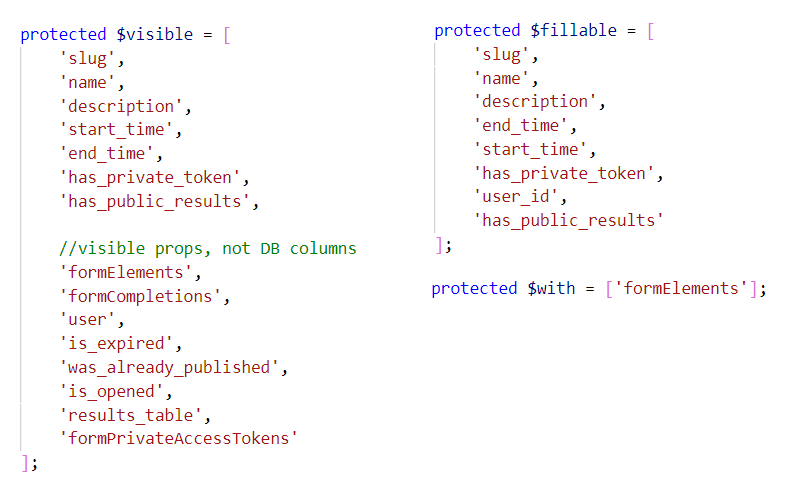
\includegraphics[width=0.8\textwidth]{img/form_model/vlastnosti.png}
		\caption{Zmíněné vlastnosti modelu formuláře}
		\label{fig:model_vlastnosti}
	\end{figure}
	
	\begin{figure}[H]
		\centering
		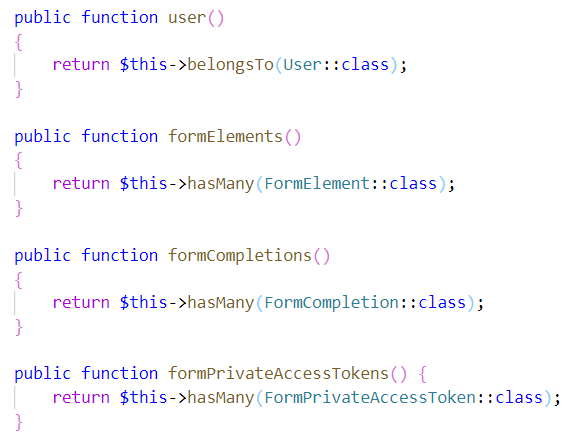
\includegraphics[width=0.65\textwidth]{img/form_model/metody.png}
		\caption{Zmíněné metody modelu formuláře}
		\label{fig:model_metody}
	\end{figure}
	%%\newpage
	
	\subsection{Kontroléry}
    Kontroléry jsou jednou z~nejdůležitějších částí celé aplikace - probíhají v~nich všechny požadované činnosti, které voláme přes specifické cesty. Obecně zajišťují veškerou administrativu nad příslušným modelem - tzn. např. model formuláře by měl mít svůj kontrolér. Většinou v~nich najdeme metody pro vrácení všech prvků nebo konkrétního prvku příslušného modelu či metody pro ukládání, aktualizaci a mazání jednotlivých prvků.
    
    Kontroléry v~této aplikaci (viz obrázek \ref{fig:kontroler}), resp. jejich metody, jsou nastaveny tak, aby v~případě chyby vrátily příslušný stavový kód pro jednoznačnou identifikaci chyby. Pokud se chyba nevyskytne, jsou navrácena příslušná data se stavovým kódem 200, který značí úspěch akce. 
    
    \begin{figure}[H]
    	\centering
    	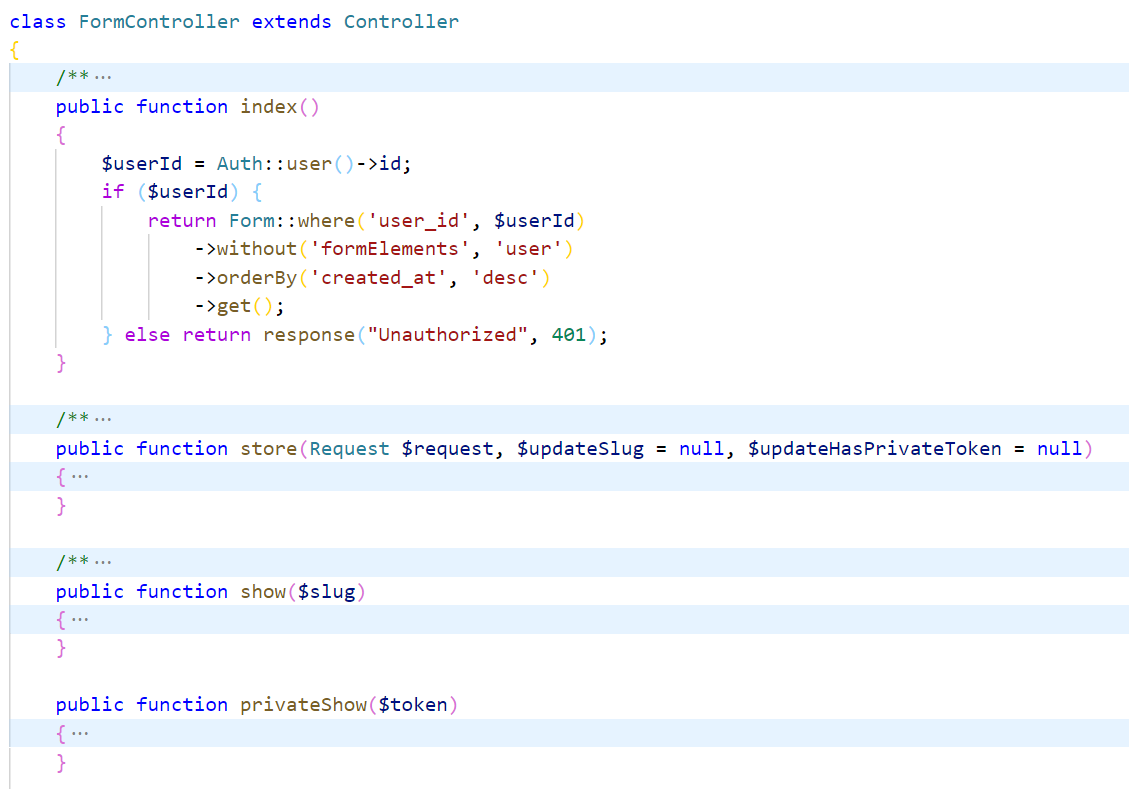
\includegraphics[width=0.85\textwidth]{img/kontroler.png}
    	\caption{Ukázka části kódu kontroléru formuláře}
    	\label{fig:kontroler}
    \end{figure}
    
    Konkrétní postupy, jak se jednotlivé činnosti provádí, jsou popsány v sekci \ref{sec:be_prubeh_jednotl_cinnosti}.
    
		\subsubsection{Kontrolér formuláře}
		Kontrolér formuláře, jak už z~názvu vyplývá, pracuje s~daty jednotlivých formulářů. Kromě výše zmíněných běžných metod obsahuje metodu pro vrácení privátního formuláře, metodu pro duplikaci formuláře, metodu pro vrácení formuláře s~dodatečnými daty pro majitele formuláře, metodu pro nastavení veřejných výsledků či metodu pro úpravu přístupu k~formuláři (nastavení veřejného nebo privátního formuláře).
		
		\subsubsection{Kontrolér vyplnění formuláře}
		Kontrolér vyplnění formuláře je oproti předchozímu kontroléru chudší. V~rámci běžných metod neobsahuje např. metodu pro úpravu či smazání odpovědi. Oproti tomu ale disponuje speciální metodou pro export všech odpovědí do stáhnutelného souboru ve formátu MS Excel, metodou pro uložení odpovědi z~privátního formuláře či metodou pro zobrazení veřejných výsledků.
		
		\subsubsection{Kontrolér uživatele}
		Kontrolér uživatele slouží ke správě uživatelů. Obsahuje základní metody pro registraci, přihlášení a odhlášení, ale i pro změnu hesla (i při zapomenutém hesle) či smazání účtu.
	
	\subsection{Exporty}\label{sec:exports}
	Exporty, resp. jejich třídy, slouží k~definování vzhledu a způsobu uložení dat v~určitém formátu. Exportovat můžeme různá data do různých formátů (např. obrázek do formátu PNG, list nějakých záznamů do tabulky formátu CSV,...).
	
	V~rámci tohoto projektu byl export potřeba jen v~jednom případě - pro exportování výsledků vyplnění formuláře pro majitele formuláře do formátu MS Excel. K~tomuto účelu byl využit přídavný balíček \uv{maatwebsite/excel}, který zajišťuje veškerou administrativu nad věcmi, které jsou s tímto úkonem spojené. Jakým způsobem jsou tato data exportována je popsáno v~sekci \ref{sec:form_comp_export}.
	
	\subsection{Maily}
	Maily, resp. jejich třídy, slouží k~definování vzhledu a obsahu emailu. Poté, co se vytvoří instance této třídy, která je hydratována (tzn. naplněna daty), jsou data předána příslušnému pohledu, který je poté poslán na požadované emaily.
	
	Způsoby a principy, kterými jsou emaily rozesílány, zde nejsou popsány - jednak jsou předdefinované Laravelem a zároveň nejsou předmětem této práce. Jediné, co bylo potřeba k~zprovoznění emailového klienta, bylo vyplnit příslušné konfigurační údaje (např. protokol pro přenos nebo port na emailový server) a přihlašovací údaje k~emailu, ze kterého jsou emaily rozesílány. K~těmto účelům byla v~implementaci projektu na produkční verzi použita bezplatná emailová služba \uv{Google Gmail}.
	
	\subsection{Migrace databáze}
	Migrace databáze jsou třídy určené k~deklaraci struktury jednotlivých tabulek v~databázi. Obecně mají dvě metody: \textit{up} pro vytvoření předdefinované tabulky a \textit{down} pro odstranění tabulky z~databáze. Tyto migrace se v~Laravelu běžně generují pomocí Artisan skriptů.~\cite{LaravelMigrace}
	
	V~implementaci tohoto projektu se využívala primárně metoda \textit{up}, kde se specifikovaly jednotlivé názvy a typy atributů tabulky (viz obrázek \ref{fig:migrace}). Těmto atributům lze přidávat další různé vlastnosti (v~migraci zapsány jako metody) jako např. \textit{nullable} (možnost vložení prázdné hodnoty \textit{null} do atributu), \textit{default} (možnost nastavení výchozí hodnoty atributu při vytvoření) či \textit{unique} (možnost nastavení unikátní hodnoty atributu ve sloupci pro celou tabulku).
	
	Kromě zmíněných vlastností bylo ještě nutné specifikovat tzv. cizí klíče, které slouží k~vytvoření relací mezi ostatními databázovými objekty a k~celkovému provázání dat. Jedná se o~samostatné atributy, které většinou obsahují ID jiného objektu v~databázi - tím je zaručeno, který řádek v~tabulce patří k~řádku/řádkům jiné tabulky. 
	
	 \begin{figure}[h]
		\centering
		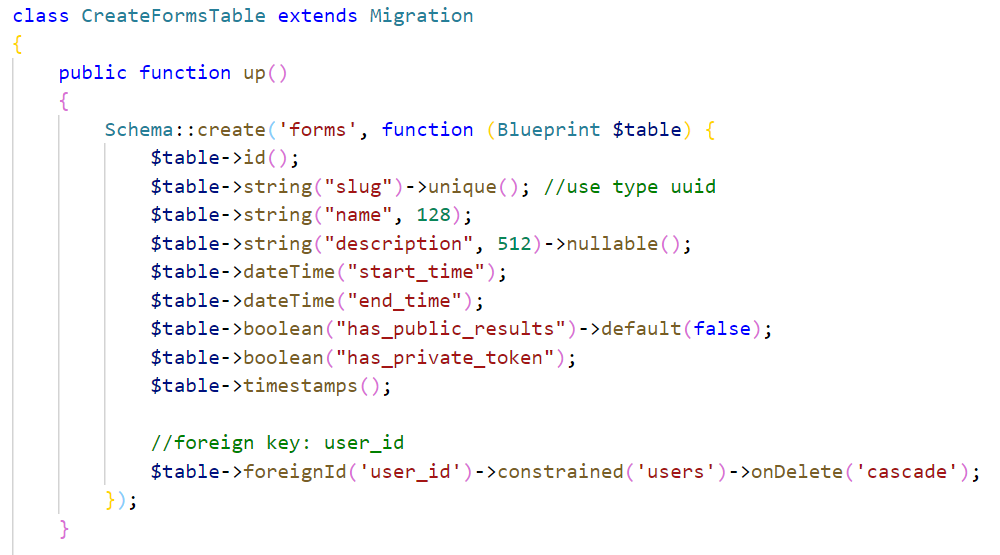
\includegraphics[width=0.85\textwidth]{img/migrace.png}
		\caption{Ukázka části kódu migrace (Tabulka pro formuláře)}
		\label{fig:migrace}
	\end{figure}
	
	V~Laravel migraci je toto deklarováno pomocí vlastnosti \textit{constrained}, ve které specifikujeme, se kterou tabulkou lze data ze současné tabulky spojovat. Pokud jsou i ostatní tabulky vytvořeny vygenerovanými migracemi, nemusíme ani specifikovat, který sloupec bude z~jiné tabulky sloužit k~provázání - k~tomu Laravel standardně používá sloupec \textit{id}.
	
	Poslední věcí, která byla nutná k~zachování referenční integrity dat v~databázi pro implementaci projektu, bylo u~několika tabulek specifikovat chování při smazání řádku z~tabulky, který je provázán s~jinou tabulkou. K~tomu slouží vlastnost \textit{onDelete}, kde toto chování deklarujeme. V~tomto projektu je použit způsob chování \uv{kaskáda}. Ta funguje v~případě mazání tak, že pokud je smazán rodičovský (nadřazený) objekt, tak jsou smazány všichni potomci (podřazené objekty) \cite{CascadeDel}.
		
		\subsubsection{Testovací data}
		K~tomu, aby bylo možné aplikaci rozumně testovat, je nutné mít v~databázi nějaká data. Pokud bychom vždy ručně tato data přidávali, trvalo by to enormní množství času - k~těmto účelům v~Laravelu existují tzv. Factories a Seeders.
		
		Factories (volně přeloženo jako Továrny) slouží k~vygenerování výplňových dat, která jsou použita primárně při vývoji aplikace. Tyto továrny na vymyšlená data jsou poté použity v~Seederu (volně přeloženo jako Rozsévač), který provádí všechny úkony jako vymazání všech současných dat databáze a následné naplnění daty z~továren.
	
	\subsection{Pohledy}\label{sec:be_pohledy}
	Pohledy jsou šablony ve formátu PHP (spravované balíčkem \uv{Blade}), pomocí kterých Laravel nativně vykresluje data uživateli. Poté, co jsou takové šabloně data předána (např. pomocí kontroléru), je šablona následně převedena na HTML formát, který je čitelný např. pro webový prohlížeč. Obvykle také obsahuje závislosti na různé přídavné soubory - např. JavaScript nebo CSS soubory. 
	
	V~tomto projektu (jak již bylo zmíněno) je pro vykreslení ve webovém prohlížeči použit pouze jeden pohled s~názvem \textit{app} (viz obrázek \ref{fig:pohled_app}). Tato šablona kromě standardní HTML hlavičky a běžných referenci na javascriptové nebo CSS soubory obsahuje pouze tělo obsahující jediný oddíl s~ID \textit{app}. Na tento oddíl díky referenci na ID poté oddělený frontend ve VueJS připojuje další jednotlivé elementy stránky - tyto elementy a další postupy jsou dále popsány ve frontendové části práce v sekci \ref{sec:impl_frontend}.
	
	\begin{figure}[h]
		\centering
		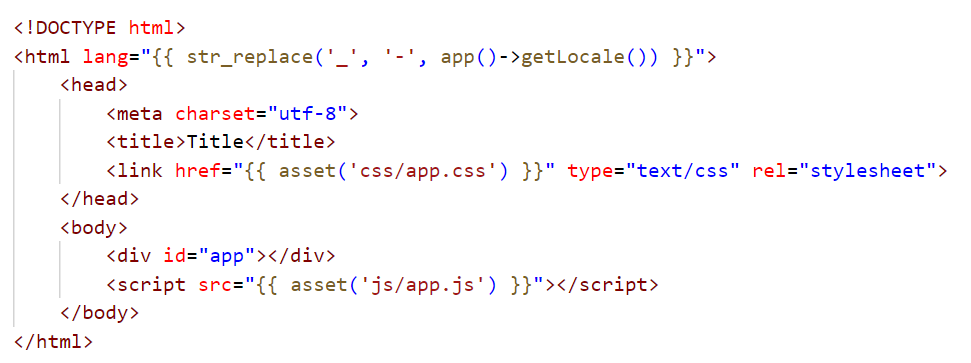
\includegraphics[width=0.9\textwidth]{img/pohled_app.png}
		\caption{Šablona pohledu \textit{app} (pro účely této práce upravena)}
		\label{fig:pohled_app}
	\end{figure}
	
	\subsection{Průběh jednotlivých činností}\label{sec:be_prubeh_jednotl_cinnosti}
	V~této části jsou popsány postupy, jak se jednotlivé akce zpracovávají na serveru a jak jsou data předávána databázi či uživateli webové stránky. Úkony jsou rozděleny tak, jak jsou zapsány v~kontrolérech. Z~hlediska kódu je každý úkon metodou kontroléru.
	
	Každá z~těchto metod vrací po provedení úkonu většinou předdefinovaný stavový kód označující, zda se činnost provedla úspěšně či nikoliv. Zde (tabulka \ref{tab:http_stavove_kody}) je seznam přímo využitých stavových kódů, které jsou serverem v této implementaci obvykle předávány.
	
	\begin{table}[H]
		\centering
		\begin{tabular}{ | p{0.1\linewidth} | p{0.3\linewidth} |  p{0.5\linewidth} |} 
			\hline
			\textbf{Stavový kód} & \textbf{Hláška} & \textbf{Popis hlášky} \\ 
			\hline
			200 & OK & Operace proběhla úspěšně. \\
			\hline
			204 & No Content & Operace proběhla úspěšně, ale žádná data nebyla klientovi poslána. \\
			\hline
			400 & Bad Request & Server nerozumí požadavku. \\
			\hline
			401 & Unauthorized & Server vyžaduje autorizaci. \\
			\hline
			404 & Not Found & Požadovaná stránka nebyla nalezena. \\
			\hline
			410 & Gone & Požadovaná stránka již není dostupná. \\
			\hline
			423 & Locked & Požadovaný zdroj je uzamčen. \\
			\hline
			500 & Internal Server Error & Obecná chybová hláška serveru - došlo k~neočekávané chybě. \\
			\hline
		\end{tabular}
		\caption{Využité stavové kódy HTTP \cite{HTTPKody1}\cite{HTTPKody2}}
		\label{tab:http_stavove_kody}
	\end{table}

	Nutno zmínit, že stavový kód \uv{200 (OK)} je v~této implementaci projektu automaticky odesílán v~případě, že není v~průběhu vyřizování požadavku zaznamenána žádná chyba. Dále v~práci proto nebude jeho odesílání zmiňováno.
	
		\subsubsection{Manipulace s~formuláři}
		Tato část popisuje veškerou administrativu nad formuláři.
		
			\subsubsubsection{Vytvoření formuláře}\label{sec:form_store}
			Metoda s~názvem \textit{store} slouží k~vytvoření a uložení formuláře s~jeho elementy do databáze. Kromě samotného vytvoření se stará o~integritu formátu jednotlivých otázek a validitu příslušných atributů formuláře. Při chybě validace předaných dat (pokud není chyba cíleně ignorována) je nejčastěji vrácen stavový kód 400.
			
			Prvním krokem, který funkce provádí, je ověření, zda je uživatel přihlášen (pokud není, je vrácen stavový kód 401). Poté se provádí rozsáhlá validace, která sestává z~kontroly základních informací o~formuláři (např. název formuláře či data zveřejněni a ukončení zveřejnění), samotných elementů formuláře a dalších parametrů validního formuláře. Před těmito úkony je zkontrolováno, zda požadavek od uživatele vůbec obsahuje nějaká data.
			
			Validace základních informací kontroluje název a popisek formuláře (zda obsahují validní řetězec, u~názvu samotné vyplnění - jedná se o~povinný atribut), data zveřejnění a ukončení zveřejnění formuláře (zda mají hodnoty správný formát, zda datum ukončení zveřejnění je dále v~čase než datum zveřejnění a zda se netvoří už expirovaný formulář s~časem ukončení zveřejnění dříve v~čase, než je aktuální serverový čas), hodnotu vyjadřující přístupnost formuláře (zda bude veřejný nebo privátní) a zda požadavek vůbec obsahuje kolekci otázek. U~privátního formuláře jsou také validovány emaily, na které se rozešle pozvánka (tzn. jejich formát).
			
			Další částí je validace elementů. Ty jsou procházeny cyklem, ve kterém se nejprve zjišťuje, zda je vybraný element elementem otázky nebo nové stránky, a kontroluje se správné pořadí na základě vlastnosti \textit{order}. Pokud se jedná o~novou stránku, přeskakuje se validace atributů otázky, a pokud má stránka validní hodnotu pro pořadí, je rovnou přemístěna mezi validní elementy. 
			
			V~případě elementu otázky je to komplikovanější. Kromě validace pořadí přichází na řadu kontroly vlastností, jako jsou typ samotné otázky (zda se jedná o~platný typ podporovaný systémem), samotný textový řetězec vyjadřující otázku (zda se jedná o~text) či atribut vyjadřující, zda se jedná o~otázku povinnou, či nikoliv (kontrola typu). Poté, na základě typu, jsou validovány atributy související s~typem otázky. Atributy, které jednotlivé typy otázek mají, jsou rozebrány v~sekci \ref{sec:form_inputs_types} - u~některých ze samotné podstaty vyplývá, co a jak se u~nich bude validovat. 
			
			Obecně platí, že u~rozsahů délky (tzn. minimální a maximální hodnoty) musí platit, že minimální hodnota je menší než maximální (a to nezávisle na typu - tzn. platí např. i pro datum - i přesto, že jsou data vkládána jako textový řetězec, musí být příslušně převedena a zvalidována). Striktní délka musí být větší než nula. U~atributů, kde má být zadána hodnota \textit{true} nebo \textit{false}, kontrolovat validní hodnotu popř. předanou hodnotu převést na validní tvar. Obvykle, pokud se nejedná o~povinnou hodnotu, se chyby ignorují - proces pokračuje dále, žádné hodnoty nejsou do těchto atributů uloženy.
			
			Nejkomplikovanější validace probíhá u~typu vstupu pro odpověď z~výběru předepsaných možných odpovědí. Zde musí být validovány i jednotlivé možnosti odpovědi pro otázku - u~nich se kontroluje počet (možností musí jich být více než dvě), zda se jedná o~škálu (na základě \textit{true}/\textit{false} hodnoty \textit{has\_hidden\_label} - pokud je tato hodnota \textit{true}, očekává se u~všech možností číselný popisek, který je pro danou kolekci možností unikátní), vnitřní pořadí (zda se jedná o~čísla tvořící posloupnost 0,1,2,3,...) a samotný text vyjadřující odpověď na otázku (zda se jedná o~platnou textovou hodnotu). V~případě selhání validace chyby nejsou ignorovány a je vrácen příslušný chybový stavový kód. Po této validaci už následuje jen validace rozsahu počtu odpovědí či striktního počtu odpovědí (pokud se jedná o~tzv. multiple-choice otázku) - u~těchto hodnot platí kromě dříve popsaných pravidel, že musí být v~symbióze s~počtem možností odpovědí - tzn. zadané hodnoty musí být menší než celkový počet možností.
			
			Po validaci zmíněných dat přichází na řadu kontrola dalších parametrů. Tím je validace pořadí (elementy musí mít v~atributu pořadí číslo, které s~ostatními tvoří posloupnost 0,1,2,3,...) a kontrola, zda v~kolekci otázek existuje alespoň jedna otázka povinná. Dále je zavedena kontrola umístění elementů nové stránky - pro ty platí, že nesmí stát na začátku a na konci kolekce elementů a že v~kolekci nesmí stát dva a více vedle sebe. V~případě výskytu chyby je vrácen příslušný chybový stavový kód.
			
			Pokud jsou všechna data validní, tak se začne vykonávat kód pro předejití poškození integrity dat v~databázové transakci, kde je v~případě tvoření formuláře nejprve vygenerován unikátní identifikátor pomocí balíčku \uv{ramsey/uuid} ve tvaru UUID4. Poté se postupně vytváří příslušné objekty pro jednotlivé prvky formuláře, kterým se předávají zvalidovaná data. Tyto objekty (resp. jejich data) jsou poté ukládány do databáze. Po tomto úkonu se v~případě privátního formuláře rozešlou pozvánky na příslušné emaily.
			
			\subsubsubsection{Úprava formuláře}\label{sec:form_update}
			Metoda s~názvem \textit{update} slouží k~editaci formuláře, který zatím nebyl zveřejněn. Díky této metodě lze kromě základních informací měnit i samotné otázky. Co v~této metodě ale nelze provést, je úprava přístupnosti formuláře a případné přidání emailů k~rozeslání pozvánky (k~tomu slouží metoda v~sekci \ref{sec:form_accessibility}).
			
			Při volání metody se nejprve ověří, zda je uživatel přihlášen (pokud není, je vrácen stavový kód 401) a zda požadovaný formulář existuje (pokud ne, je vrácen stavový kód 404). Poté přichází na řadu kontrola časů - kontroluje se, zda už nebyl formulář zveřejněn na základě data zveřejnění formuláře (atribut musí být dále v~čase než je serverový čas). Pokud tato podmínka není splněna, je vrácen stavový kód 400.
			
			Dále je spuštěna databázová transakce, ve které se nejprve vygeneruje dočasný identifikátor \textit{slug} formuláře ve tvaru UUID4. Poté se všechna data z~požadavku uživatele předají metodě \textit{store} (popsána v~sekci \ref{sec:form_store}), která přidá do databáze formulář s~předanými úpravami. Kromě dat z~požadavku se metodě poskytnou i další data: dočasný identifikátor, který slouží k~identifikaci přidaného upraveného formuláře a informace o~tom, zda byl upravovaný formulář veřejný nebo privátní. Dočasný identifikátor je použit místo vygenerovaného identifikátoru použitého přímo v~metodě \textit{store}. Předávaná informace o~přístupnosti slouží k~tomu, aby upravený formulář tuto vlastnost neztratil a aby nebyly znovu rozeslány pozvánky na příslušné emaily, což je nativní chování metody \textit{store}. 
			
			Poté, pokud nebyl uživatelský požadavek validní dle metody pro přidání formuláře, je vrácen příslušný stavový kód pocházející přímo ze zmíněné metody. Pokud ale vše v~metodě \textit{store} proběhlo bez problému, následují další činnosti. 
			
			Pokud se jedná o~veřejný formulář, původní (neupravený) formulář (a s~ním i další objekty na něj navázané) je smazán pomocí metody \textit{destroy} (popsána v~sekci \ref{sec:form_destroy}) a u~upraveného formuláře je přepsán identifikátor na hodnotu identifikátoru, kterou disponoval neupravený formulář. V~případě, že je upravený formulář privátní, se prvně do dočasné proměnné uloží všechny přístupové tokeny. Poté se původní formulář smaže a nahradí se identifikátor stejně jako u~veřejného formuláře. Nakonec se vytvoří kopie tokenů na základě dat v~dočasné proměnné zmíněné dříve, které se liší jen v~hodnotě ID formuláře (to, jelikož byl de facto vytvořen nový formulář, musí odkazovat na upravený formulář). Při neočekávaných chybách je vrácen stavový kód 500.
			
			\subsubsubsection{Duplikování formuláře}\label{sec:form_dupl}
			Metoda s~názvem \textit{duplicateWithAuth} slouží k~duplikování formuláře - tzn. lze vytvořit nový formulář, který obsahuje stejné otázky a vlastnosti (tj. jméno formuláře, datum zveřejnění, datum ukončení zveřejnění,...), jako formulář, u~kterého byla požadována duplikace. Zmíněné vlastnosti při tomto procesu lze modifikovat, otázky ne.
			
			Metoda funguje tak, že prvně ověří, zda je uživatel přihlášen (pokud ne, vrátí stavový kód 401), poté zkontroluje zda požadovaný formulář existuje a zda patří přihlášenému uživateli. Dále jsou validovány všechny předané hodnoty vlastností formuláře, které již byly zmíněné - tzn. zda vůbec v~požadavku na duplikaci existují a zda jsou správného typu (v~případě jakékoliv očekávané chyby je vrácen kód 400). 
			
			U~hodnot pro čas zveřejnění a ukončení zveřejnění se validuje příslušný formát data, zda není čas zveřejnění větší (déle v~čase) než čas ukončení zveřejnění či zda není vytvářen už expirovaný formulář (tzn. aktuální serverový čas je déle v~čase než čas ukončení zveřejnění). 
			
			Poté probíhá kontrola nastavení přístupnosti formuláře - při duplikaci lze změnit tento atribut. Pokud je tento atribut nastaven jako \textit{true} (tzn. formulář je privátní, lze k~němu přistupovat jen s~tokenem), kontrolují se předané emaily (zda mají validní tvar), na které se bude rozesílat pozvánka.
			
			Nakonec se vygeneruje nový identifikátor ve tvaru UUID4 a metoda se pokouší příslušná data uložit do databáze. Zde vzniká nový objekt formuláře, kterému jsou předány příslušné vlastnosti (tj. ID uživatele, vygenerovaný identifikátor a data z~požadavku duplikace). S~tím podobně vznikají i příslušné objekty pro uložení jednotlivých elementů formuláře (tj. otázky nebo nové stránky), jejichž vlastnosti jsou přebírány a kopírovány z~duplikovaného formuláře. Nakonec, pokud je formulář nastaven jako privátní, jsou rozeslány pozvánky na zvalidované emaily. Tento proces probíhá v~databázové transakci.
			
			Při úspěchu je vrácena odpověď s~identifikátorem nově vzniklého formuláře (duplikátu). Ten je určen pro frontendovou část projektu k~přesměrování.
								
			\subsubsubsection{Úprava přístupnosti formuláře}\label{sec:form_accessibility}
			Metoda s~názvem \textit{updateAccess} slouží k~úpravě přístupnosti formuláře. V~ní lze nastavit, zda je formulář veřejný, nebo privátní (s~tím je možné nastavit, na které emaily lze dodatečně poslat pozvánku či kterým emailům s~pozvánkou odebrat přístup ve formě invalidace tokenu).
			
			V~rámci zpracování dat je nejprve kontrolováno, zda požadavek obsahuje vůbec nějaká data (pokud ne, je vrácen stavový kód 400). Poté se kontroluje přihlášení uživatele (pokud není přihlášen, je vrácen stavový kód 401) a zda požadovaný formulář s~příslušným vlastníkem existuje (pokud ne, je vrácen stavový kód 404). Další akce jsou prováděny jen pokud existuje v~požadavku uživatele atribut \textit{has\_private\_token} s~platnou hodnotou (pokud neexistuje, je vrácen stavový kód 400). Po těchto kontrolách se dále celý proces dělí na dvě logické větve. 
			
			První větev je podmíněna tím, že se zmíněný předaný atribut \textit{has\_private\_token} se rovná \textit{true} (tzn. formulář bude privátní). V~takovém případě se nejprve zvalidují předané emaily, na které má být odeslána nová pozvánka (pokud dojde k~chybě ve validaci samotných emailů, je vrácen kód 400). Poté, pokud byl měněný formulář veřejný (tzn. před tímto úkonem se jeho hodnota \textit{has\_private\_token} rovnala \textit{false}), se formuláři v~databázi přepisuje zmíněný atribut \textit{has\_private\_token} na \textit{true} a vytváří se nové tokeny pro předané emaily, na které je poté rozeslána pozvánka. Pokud byl ale měněný formulář už privátní, tak jsou, společně s~vytvořením nových tokenů a rozesláním pozvánek, zneplatněny pozvánky, které byly zaslané na majitelem předané emaily - tzn. po validaci těchto dat jsou z~databáze vymazány tokeny, ke kterým jsou vázány příslušné emaily z~uživatelského požadavku. Uživatelům, kterým byla pozvánka zneplatněna, se žádný oznamovací email nezasílá.
			
			Druhá větev je podmíněna tím, že zmíněný předaný atribut \textit{has\_private\_token} se rovná \textit{false} a atribut požadovaného formuláře \textit{has\_private\_token} se rovná \textit{false} (tzn. formulář bude převeden na veřejný). V~takovém případě proběhne triviální smazání všech privátních tokenů, které se na příslušný formulář váží. Žádný oznamovací email se uživatelům s~pozvánkou neposílá.
			
			Veškeré databázové operace spojené se zmíněnými úkony probíhají pro zachování integrity dat v~transakcích.
			
			\subsubsubsection{Zveřejnění výsledků formuláře}\label{sec:form_publish_results}
			Metoda s~názvem \textit{publishResults} slouží k~modifikaci přístupu k~výsledkům formuláře pro běžnou veřejnost. Zde lze nastavit, zda jsou výsledky veřejné či nikoliv. Pokud jsou výsledky zveřejněny, lze zvolit, které otázky jsou skryté a které jsou zveřejněné.
			
			Funkce nejprve zkontroluje, zda požadavek obsahuje vůbec nějaká data (pokud ne, je vrácen stavový kód 400). Poté kontroluje přihlášení uživatele (pokud není přihlášen, je vrácen stavový kód 401) a zda požadovaný formulář s~příslušným vlastníkem existuje (pokud ne, je vrácen stavový kód 404). Po těchto kontrolách jsou validována předaná data v~požadavku na server.
			
			V~rámci zmíněných dat se nejprve validuje předaný atribut \textit{has\_public\_results}, který stanovuje, zda má formulář veřejné výsledky - tzn. zda má platnou hodnotu. Poté, pokud je předchozí hodnota \textit{true} (tzn. výsledky budou zveřejněny), jsou procházena a validována všechna data z~uživatelova požadavku, která představují jednotlivé otázky a jejich atribut zveřejnění. Zde se kontroluje, zda otázky vůbec náleží požadovanému formuláři (pomocí \textit{id}) - pokud ano, jsou dále předávány společně s~informací, zda mají být tyto otázky veřejné, nebo ne (neplatná data v~této části jsou ignorována). Zároveň musí platit, že v~případě zveřejnění výsledků formuláře musí být alespoň jedna otázka veřejná (pokud toto neplatí, je vrácen stavový kód 400).
			
			Poté se metoda pokouší tato data uložit do databáze. Nejprve přepisuje atribut formuláře \textit{has\_public\_results}, poté, na základě tohoto atributu, manipuluje s~jednotlivými elementy. Pokud je zmíněný atribut \textit{true}, tak jsou jednotlivé elementy modifikovány podle zvalidovaných dat (tzn. pokud mají být veřejné, je jim nastaven stejnojmenný atribut \textit{has\_public\_results} na true, v~opačném případě na \textit{false}). Pokud je ale zmíněný atribut formuláře \textit{false}, je všem elementům zmíněný atribut zveřejnění nastaven na \textit{false} (tzn. všechny odpovědi jsou skryty). Celý proces probíhá v~transakci.
			
			\subsubsubsection{Mazání formuláře}\label{sec:form_destroy}
			Metoda s~názvem \textit{destroy} slouží k~odstranění formuláře a jeho přidružených elementů.
			
			V~koncepci je metoda velice jednoduchá - poté, co se zkontroluje, zda je uživatel přihlášen (pokud ne, je vrácen stavový kód 401) a zda vůbec formulář s~předaným \textit{slug} identifikátorem patřící přihlášenému uživateli v~databázi existuje (pokud ne, je vrácen stavový kód 404), je pomocí příslušné nativní metody \textit{delete} smazán. Tento proces také probíhá v~transakci.
			
			\subsubsubsection{Vrácení všech formulářů uživateli}\label{sec:form_index}
			Metoda s~názvem \textit{index} je určena k~vrácení všech formulářů, které patří přihlášenému uživateli. To slouží k~hydrataci úvodní stránky uživatele - jedná se o~přehled všech vlastněných formulářů. 
			
			Tato funkce nejprve ověří, zda je uživatel přihlášen. Pokud přihlášen je, vrátí uživateli všechny jeho formuláře bez elementů formuláře a bez dat o~uživateli, které se obecně k~datům připojují. Tento set formulářů je seřazen podle doby vytvoření formuláře sestupně. Pokud přihlášen není, je vrácen stavový kód 401. 
			
			\subsubsubsection{Vrácení informací o~formuláři majiteli}\label{sec:form_showwithauth}
			Metoda s~názvem \textit{showWithAuth} má za účel vrátit celý formulář a data s~ním spojená pro jeho vlastníka. Tato data poté slouží k~hydrataci stránky s~přehledem informací o~formuláři.
			
			Funkce nejprve zkontroluje, zda je uživatel přihlášen. Pokud není, je navrácen stavový kód 401. V~případě, že je uživatel přihlášen, se v~databázi vyhledává formulář na základě předaného identifikátoru \textit{slug}. Pokud formulář není nalezen, je vrácen stavový kód 404, a pokud nepatří přihlášenému uživateli, je vrácen kód 401. 
			
			Po zmíněných kontrolách se k~objektu formuláře připojují tři atributy: \textit{is\_expired} (rovná se \textit{true}, pokud je serverový čas dále v~čase než čas ukončení zveřejnění), \textit{was\_already\_published} (rovná se \textit{true}, pokud je serverový čas dále v~čase než čas zveřejnění formuláře) a \textit{is\_opened} (rovná se \textit{true}, když neplatí \textit{is\_expired} a zároveň platí \textit{was\_already\_published} - tzn. když je formulář dostupný k~vyplnění). Po připojení těchto vlastností je celý formulář s~příslušnými vlastnosti vrácen.
			
			Pokud je formulář nastaven jako privátní, tak jsou k~celému objektu formuláře ještě připojeny záznamy o~privátních tokenech. Tyto záznamy slouží pro vlastníka formuláře k~výpisu emailů, kterým byla poslána pozvánka a které mají v~době vykonávání této metody oprávnění k~vyplnění formuláře. Připojené záznamy o~tokenech samotný token neobsahují (resp. je skrytý pro vlastníka formuláře) - to slouží k~tomu, aby nebylo možné dohledat, který token patří ke kterému emailu. Zároveň to znemožňuje jednoduše odpovědět za člověka, kterému byla odeslána pozvánka k~vyplnění.
			
			\subsubsubsection{Vrácení konkrétního veřejného formuláře}\label{sec:form_show}
			Metoda s~názvem \textit{show} je určena k~vrácení konkrétního veřejného formuláře. To slouží k~hydrataci stránky určené k~vyplnění veřejného formuláře.
			
			V~rámci celého procesu funkce nejprve ověří, zda v~databázi existuje formulář s~požadovaným identifikátorem \textit{slug}. Pokud ne, je vrácen stavový kód 404. Pokud ale nalezen je, provádí se několik kontrol - když kontrolami projde, je navrácen formulář s~příslušnými elementy.
			
			První se kontroluje, zda zadaný identifikátor neukazuje na privátní formulář - na tento formulář lze přistoupit jen přes token, nikoliv přes zmíněný identifikátor. Pokud se potvrdí přístup přes identifikátor, odešle se jen stavový kód 400.
			
			Dalším faktorem je čas, kdy k~formuláři chce uživatel přistoupit. Ověřuje se podle uložených dat o~formuláři z~databáze, zda je už formulář zveřejněn (pokud není, je vrácen stavový kód 423), nebo zda už formulář neexpiroval (pokud expiroval, je vrácen stavový kód 410). Aktuální čas se bere podle serveru, na kterém je aplikace nasazena.
			
			\subsubsubsection{Vrácení konkrétního privátního formuláře}\label{sec:form_privateshow}
			Metoda s~názvem \textit{privateShow} funguje podobně jako metoda \textit{show} popsaná v~sekci \ref{sec:form_show} a slouží k~hydrataci stránky určené k~vyplnění privátního formuláře. 
			
			Oproti zmíněné předchozí metodě se místo identifikátoru \textit{slug} nejprve vyhledává uživatelem předaný token v~databázi. Pokud nalezen není, je vrácen stavový kód 400. Pokud nalezen je, provádí se stejné kontroly časů jako v~metodě v~sekci \ref{sec:form_show}. Liší se ale v~kontrole tokenu - zde je zjišťováno, zda není token už expirovaný resp. zda už pro tento token nebyla zaznamenána odpověď. Pokud expirovaný je, tak se odesílá jen stavový kód 410. Pokud požadavek na privátní formulář projde bez chyby, je odeslán formulář s~příslušnými elementy - identifikátor \textit{slug} se pro koncového uživatele skrývá.
 
		\subsubsection{Interakce s~odpovědmi na formuláře}
		Tato část popisuje veškerou administrativu nad zaznamenáváním odpovědí k~formuláři.
		
			\subsubsubsection{Zaznamenávání odpovědi na veřejný formulář}\label{sec:form_comp_public}
			Metoda s~názvem \textit{store} slouží k~zaznamenání všech odpovědí na příslušný veřejný formulář. V~případě očekávané chyby je nejčastěji vrácen chybový kód 400 - proto dále v~textu není zmiňován.
			
			První věcí, která se provádí, je ověření, zda existuje formulář, na který lze odpovědět, na základě předaného identifikátoru \textit{slug} (v~případě této chyby je vrácen stavový kód 404). Také se kontroluje, zda se nejedná o~privátní formulář - na ten nelze přes identifikátor odpovědět (k~tomu je určena metoda \textit{privateStore} popsána v~sekci \ref{sec:form_comp_private}). Dále se kontroluje, zda je formulář už zveřejněný a zároveň zda není expirovaný (serverový čas v~okamžiku, kdy je odeslána odpověď, musí být v~intervalu mezi datem zveřejnění a datem ukončení zveřejnění). Po těchto operacích je formulář uložen v~dočasné proměnné pro další úkony popsané níže.
			
			Poté je inicializována vnitřní metoda \textit{getCorrespondingValue} sloužící k~nalezení příslušných dat a ucelení formátu předaných informací z~požadavku na server. Té jsou předávány tyto parametry: \textit{request} (celý požadavek od uživatele), \textit{type} (řetězec identifikující typ otázky) a \textit{specificInputId} (\textit{id} otázky, pro kterou je hledána odpověď). Metoda na základě předaných dat projde celý požadavek, ve kterém jednotlivé záznamy odpovědí zpracuje (tzn. zkontroluje jejich formát). Pokud je formát platný, testují se proti sobě příslušná data z~požadavku a předaná data v~parametrech metody (tzn. zda se typ a ID otázky z~požadavku a z~parametru rovnají). Pokud je nalezena taková shoda, jsou vrácena data (tj. ID otázky, typ otázky a předaná hodnota/odpověď) připravená ve formátu asociativního pole určená k~další validaci. Pokud shoda nalezena není, jsou vrácena stejná data, jen bez předané hodnoty (pro případy otázek, u~kterých není odpověď povinná).
			
			Dále jsou cyklem procházeny všechny elementy zodpovězeného formuláře. Cyklus postupně zkouší najít příslušnou hodnotu pro každou otázku. Krok cyklu je větven do několika částí, které se odvíjejí od typu otázky. V~každé větvi je poté, na základě známého typu otázky, prohledáván požadavek od uživatele pomocí metody \textit{getCorrespondingValue} k~nalezení příslušné odpovědi, která je převedena do pracovního formátu. Ta je poté validována podle předepsaných pravidel příslušné otázky, jež byla deklarována při tvoření formuláře (např. maximální délka předané textové odpovědi) v~metodě \textit{store} ze sekce \ref{sec:form_store} - tzn. pokud je povinná, musí mít platnou hodnotu, pokud povinná není, může mít kromě platné hodnoty hodnotu \textit{null}. Komplikovanější, ale v~podstatě stejná, je validace vstupu pro odpověď z~výběru předepsaných možných odpovědí, kde se podobně jako v~metodě \textit{getCorrespondingValue} v~dalším vnořeném cyklu testují i příslušné možnosti odpovědi (zda vůbec k~formuláři patří a zda se jedná o~platnou hodnotu).
			
			Po tomto validačním procesu následuje databázová transakce, ve které se celá odpověď ukládá do databáze. Pro celou odpověď je nejprve vytvořen záznam o~vyplnění formuláře, kterému je předáno ID formuláře, na který byla odpověď směřována. Poté se vytváří na základě validního setu odpovědí k~příslušným vstupům příslušné databázové objekty, které jsou zaobaleny záznamem o~vyplnění formuláře a do databáze uloženy.
			
			\subsubsubsection{Zaznamenávání odpovědi na privátní formulář}\label{sec:form_comp_private}
			Metoda s~názvem \textit{privateStore} slouží k~zaznamenání všech odpovědí na privátní formulář.
			
			V~rámci funkčnosti je tato metoda opravdu velmi spjatá s~metodou popsanou v~sekci \ref{sec:form_comp_public}. Prvním krokem je ověření, zda použitý přístupový token existuje (pokud ne, je vrácen stavový kód 400) a zda pomocí tohoto tokenu už nebyla zaznamenána odpověď (pokud ano, je vrácen stavový kód 410). Poté se na základě předaného tokenu musí vyhledat formulář, kterému token náleží, a z~něj získat jeho identifikátor \textit{slug}. Následuje použití metody \textit{store} ze sekce \ref{sec:form_comp_public} - té je předán celý uživatelský požadavek, identifikátor nalezený v~předchozím kroku a informace o~tom, že se odpovídá na privátní formulář (metoda standardně počítá s~tím, že se odpovídá na veřejný formulář, takže bez předání této informace by odpověď blokovala). Na základě stavového kódu z~vnitřně volané metody \textit{store} se provádí další činnosti. 
			
			V~případě, že byla odpověď zaznamenána úspěšně (byl vrácen stavový kód 200), se v~databázové transakci přepíše atribut tokenu, který vyjadřuje, že už pomocí něho byla zaznamenána odpověď, na hodnotu \textit{true} (tzn. byl použit, nelze s~tímto tokenem dále odpovídat). Pokud se ale vyskytla chyba v~průběhu metody \textit{store}, tak je uživateli vrácen touto metodou předaný chybový kód.
			
			\subsubsubsection{Vrácení všech výsledků}\label{sec:form_comp_private_index}
			Metoda s~názvem \textit{index} slouží k~vypsání všech odpovědí na formulář majiteli požadovaného formuláře.
			
			Funguje tak, že po kontrole autentizace (u~chyby vrácen stavový kód 401) a autorizace (u~chyby vrácen stavový kód 404) se k~nalezenému formuláři postupně připojí všechny existující odpovědi k~příslušným typům otázek pomocí vazeb, které lze vytvářet na Laravel modelech (viz obrázek \ref{fig:vraceni_vsech_vysledku}). Poté, pokud byla nalezena alespoň jedna odpověď na formulář, je vrácen celý objekt formuláře, ke kterému je připojen set dat obsahující všechny odpovědi. Pokud nebyla zaznamenána žádná odpověď, je vrácen stavový kód 204 (nejedná se o~chybu, jen neexistují žádná data k~předání).
			
			\begin{figure}[h]
				\centering
				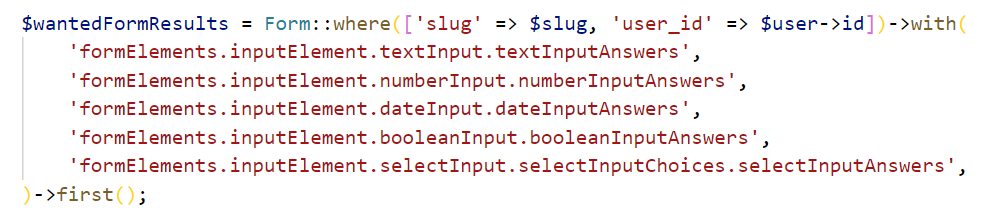
\includegraphics[width=0.9\textwidth]{img/vraceni_vsech_vysledku.png}
				\caption{Ukázka části kódu metody \textit{index} pro získání odpovědí na formulář}
				\label{fig:vraceni_vsech_vysledku}
			\end{figure}
			
			\subsubsubsection{Vrácení veřejných výsledků}\label{sec:form_comp_public_index}
			Metoda s~názvem \textit{publicIndex} slouží k~vypsání všech odpovědí na formulář. Tento výpis je dostupný jen v~případě, že majitel formuláře tuto funkci aktivoval (popsáno v~sekci \ref{sec:form_publish_results}) - poté jsou vybrané výsledky dostupné pro kohokoliv. 
			
			Tato metoda funguje velmi podobně jako metoda \textit{index} popsaná v~sekci \ref{sec:form_comp_private_index}. Oproti zmíněné metodě nekontroluje přihlášení uživatele, ale zda jsou výsledky dotazovaného formuláře nastaveny jako veřejné. Z~podstaty věci také omezuje viditelnost vybraných otázek na základě hodnoty \textit{has\_public\_results}, kterou musí disponovat všechny otázky - pokud je nastavena na \textit{false}, tak je otázka z~výstupního setu odebrána. Pokud jsou všechny nastaveny jako skryté, odesílá se stejný stavový kód jako při situaci, kdy neexistuje žádná odpověď na formulář. Jinak se tato metoda oproti zmíněné metodě \textit{index} neliší.
			
			\subsubsubsection{Export výsledků}\label{sec:form_comp_export}
			Metoda s~názvem \textit{export} je určena k~exportování všech odpovědí do souboru formátu MS Excel (s~příponou .xlsx). Tato data mají sloužit při správném nastavení formuláře a jeho odpovědí např. ke korelační analýze (především u~škálových typů otázek). K~tomuto úkonu je použit přídavný balíček \uv{maatwebsite/excel} (především třída \textit{Excel}), který po předání příslušných dat celý exportní proces obstarává (viz sekce \ref{sec:exports}).
			
			Metoda funguje tak, že nejprve volá metodu \textit{index} (popsána v~sekci \ref{sec:form_comp_private_index}), které předává identifikátor formuláře z~uživatelského požadavku. Poté, pokud je ze zmíněné metody navrácen objekt formuláře (tzn. že celý proces proběhl úspěšně - byla předána platná kolekce odpovědí), jsou příslušná data předána metodě \textit{download} na statické třídě \textit{Excel}, která vygeneruje příslušný soubor. Pokud je z~metody \textit{index} vrácen jen stavový kód, tak je uživateli předán společně s~příslušnou chybovou hláškou.
			
			Samotný export dat je proveden tak, že se zmíněné metodě \textit{download} předá instance objektu, která zaobaluje předaná data k~exportu a definuje, jak budou v~souboru sázena. Metoda \textit{download} poté vytvoří soubor, který je poslán uživateli. Instance objektu je tvořena ze třídy \textit{FormCompletionsExport}, která byla k~tomuto účelu připravena - implementuje rozhraní \textit{FromArray} (z~balíčku pro export) a obsahuje příslušnou metodu \textit{array}, která vybraná data zpracovává a vrací ve formě pole polí (reprezentuje sloupce a řádky v~tabulce). Metoda určuje formát dat takto (viz obrázek \ref{fig:export_excel}):
			
			\begin{itemize}
				\item Na prvním řádku v~první buňce (roh tabulky) je umístěn samotný název formuláře.
				\item Na druhém řádku je nejprve definován sloupec \textit{Completion ID} (ten obsahuje ID pro každou zaznamenanou odpověď - jedná se o~\textit{id} databázového objektu pro vyplnění formuláře viz sekce \ref{sec:form_completions}). Poté jsou v řádku sázeny jednotlivé otázky formuláře.
				\item Na dalších řádcích jsou vypsána data z~odpovědi - tzn. na prvním místě ID vyplnění formuláře, poté příslušné odpovědi pod příslušnými otázkami.
			\end{itemize}
		
			\begin{figure}[h]
				\centering
				
\includegraphics[width=0.95\textwidth]{img/export_excel.png}
				\caption{Ukázka vyexportovaných dat (pro potřeby této práce upraveno)}
				\label{fig:export_excel}
			\end{figure}
		
			Zpracování odpovědí nejprve probíhá tak, že se shromáždí všechna ID vyplnění formuláře pro požadovaný formulář - tím se vytvoří připravené \uv{chlívečky} pro odpovědi (jednorozměrné pole), které jsou od sebe oddělené právě pomocí ID vyplnění formuláře (co \textit{chlíveček}, to řádek s~odpovědmi). Dále se na první index \uv{chlívečku} umístí samotné ID vyplnění. Poté se prochází jednotlivé odpovědi, které se postupně ukládají do zmíněných \uv{chlívečků}, přičemž je dbáno na to, aby se odpovědi ukládaly pod správné otázky. U~otázek s~možnostmi odpovědí v~případě multiple-choice jsou data rozdělována středníkem. Pokud je otázka nepovinná a nebyla zodpovězena, buňka ve výstupu bude prázdná. 
			
			Nakonec se otázky rozmístěné do \uv{chlívečků} ještě upraví (tzn. kde se nachází logické hodnoty \textit{true} nebo \textit{false}, tam je umístěn textový ekvivalent \uv{true} nebo \uv{false}). Podobná úprava probíhá i u~samotných otázek v~2. řádku tabulky (pokud je otázka povinná, je jí na konec přidán znak hvězdičky \uv{*}).
			
		\subsubsection{Interakce s~uživateli}
		Tato část popisuje veškerou administrativu nad uživatelskými účty. Nutno zmínit, že v~projektu byly pro tyto účely použity nativní materiály a funkce Laravelu (např. model uživatele, migrace tabulky uživatelů a validační funkce). V~rámci validačních funkcí zde nebudou popsány stavové kódy, které při chybě vracejí, jelikož se jedná o~funkcionalitu spravovanou přímo frameworkem Laravel.
		
			\subsubsubsection{Registrace uživatele}\label{sec:user_register}
			Metoda \textit{register} slouží k~vytvoření nového uživatelského účtu.
			
			V~rámci funkčnosti metoda nejdříve přijme požadavek od uživatele, ve kterém očekává určité parametry (přezdívka uživatele, email, heslo a potvrzení hesla). Pokud tyto parametry dostane a jsou platné (tzn. že splňují požadavky jako že se jedná o~platné textové hodnoty, že email musí být u~uživatele unikátní a že je heslo alespoň 8 znaků dlouhé), vytvoří se hash hesla (to je zašifrováno pomocí funkce \textit{bcrypt}) a všechna data o~uživateli se uloží do databáze. 
			
			\subsubsubsection{Přihlášení uživatele}\label{sec:user_login}
			Metoda \textit{login} slouží k~přihlášení uživatele k~uživatelskému účtu. 
			
			Funkce funguje tak, že nejprve (podobně jako v~metodě \textit{register} v~sekci \ref{sec:user_register}) zvaliduje příchozí data (zde email a heslo) a až poté, co se ověří, že jsou údaje platné (pomocí statické třídy \textit{Auth}), se odesílá objekt s~daty o~přihlášeném uživateli.
			
			\subsubsubsection{Odhlášení uživatele}\label{sec:user_logout}
			Metoda \textit{logout} slouží k~odhlášení uživatele - tedy k~invalidování relace. Obsahuje jen volání metody \textit{logout} na statické třídě \textit{Auth}, která zařizuje veškerou administrativu nad přihlášenými uživateli a tedy i nad tímto úkonem.
			
			\subsubsubsection{Vrácení informací o~uživateli}\label{sec:user_show}
			Metoda \textit{show} přihlášenému uživateli vrátí data o~jeho účtu resp. jeho osobní údaje jako je např. přezdívka nebo email.
			
			Funguje tak, že pokud je uživatel přihlášen, jsou jednoduše vrácena jeho osobní data z~databáze. Pokud není přihlášen, je vrácen stavový kód 401.
			
			\subsubsubsection{Vymazání účtu uživatele}\label{sec:user_destroy}
			Metoda \textit{destroy} slouží k~odstranění uživatelského účtu na základě požadavku vlastníka profilu. Vlastník k~tomuto úkonu samozřejmě musí být přihlášen.
			
			Jelikož k~tomuto úkonu musí být předáno současné heslo k~účtu, je prvně kontrolováno právě to resp. jestli se jedná o~validní textový řetězec. Poté je zjišťováno, zda je vůbec nějaký uživatel přihlášen (pokud není, je vrácen stavový kód 400). Pokud ano, je kontrolováno, zda se heslo shoduje s~heslem v~databázi (pokud ne, je vrácen stavový kód 400). Pokud se hesla shodují, je uživatel z~databáze smazán.
			
			\subsubsubsection{Změna hesla}\label{sec:user_changepassword}
			Metoda \textit{changePassword} slouží ke změně hesla za předpokladu, že uživatel stávající heslo zná.
			
			V~rámci průběhu celého úkonu metody, prvně se kontroluje, zda je vůbec nějaký uživatel přihlášen. Pokud není, je vrácen stavový kód 401. Pokud ale přihlášen je, tak nejprve dochází k~validaci dat (podobně jako v~sekci \ref{sec:user_register}). Dále se kontroluje, zda je původní heslo shodné s~předaným původním heslem, zda není staré a nové heslo stejné a zda je nové heslo shodné s~potvrzením tohoto hesla. Pokud všemi kontrolami projde, dochází k~vytvoření nového hashe hesla, kterým je přepsán starý hash uživatele.
			
			\subsubsubsection{Resetování zapomenutého hesla uživatele} \label{sec:user_reset_forgot_password}
			Tento proces je obhospodařován dvěma metodami - \textit{forgotPassword} a \textit{resetPassword}. Celý proces resetování hesla probíhá tak, že uživatel odešle požadavek na metodu \textit{forgotPassword}, která mu na jeho email pošle odkaz k~resetování hesla - ten vede na stránku, kde si zvolí nové heslo. Poté, co nové heslo vyplní, odesílá požadavek na metodu \textit{resetPassword}, která heslo za splnění všech podmínek (tj. validace dat a správnost obnovovacího tokenu) změní. 
			
			Metoda \textit{forgotPassword} tedy v~požadavku přijímá jen email, který je nejprve validován. Poté je na něj odeslán odkaz k~resetování hesla. Pokud se odeslání nezdaří, je vrácen stavový kód 400.
			
			K~metodě \textit{resetPassword} je přistupováno právě z~odkazu poslaného pomocí metody \textit{forgotPassword}. Metoda \textit{resetPassword} přijímá ověřovací token předaný v~odkazu v~emailu, samotnou emailovou adresu a heslo s~potvrzením. Pokud jsou předaná data validní, je vygenerován nový hash hesla, který přepíše stávající hash. Pokud se při resetování hesla vyskytne chyba, je vrácen stavový kód 400.
			

